\documentclass{article}%
\usepackage[T1]{fontenc}%
\usepackage[utf8]{inputenc}%
\usepackage{lmodern}%
\usepackage{textcomp}%
\usepackage{lastpage}%
\usepackage[head=40pt,margin=0.5in,bottom=0.6in]{geometry}%
\usepackage{graphicx}%
%
\title{\textbf{Programa Mundial de Alimentos necesita \$22 millones para atender a venezolanos que entran a Colombia}}%
\author{EFE}%
\date{25/09/2018}%
%
\begin{document}%
\normalsize%
\maketitle%
\textbf{URL: }%
http://www.eluniversal.com/politica/21514/programa{-}mundial{-}de{-}alimentos{-}necesita{-}22{-}millones{-}para{-}atender{-}a{-}venezolanos{-}que{-}entran{-}a{-}colombia\newline%
%
\textbf{Periodico: }%
EU, %
ID: %
21514, %
Seccion: %
politica\newline%
%
\textbf{Palabras Claves: }%
NO\_TIENE\newline%
%
\textbf{Derecho: }%
2.10, %
Otros Derechos: %
CONTEXTO, %
Sub Derechos: %
2.10.1\newline%
%
\textbf{EP: }%
NO\newline%
\newline%
%
\textbf{\textit{La falta de alimentos se convierte en el principal problema para quienes atraviesan a diario la frontera entre Venezuela y Colombia, que cuenta con siete puntos de pasaje oficiales}}%
\newline%
\newline%
%
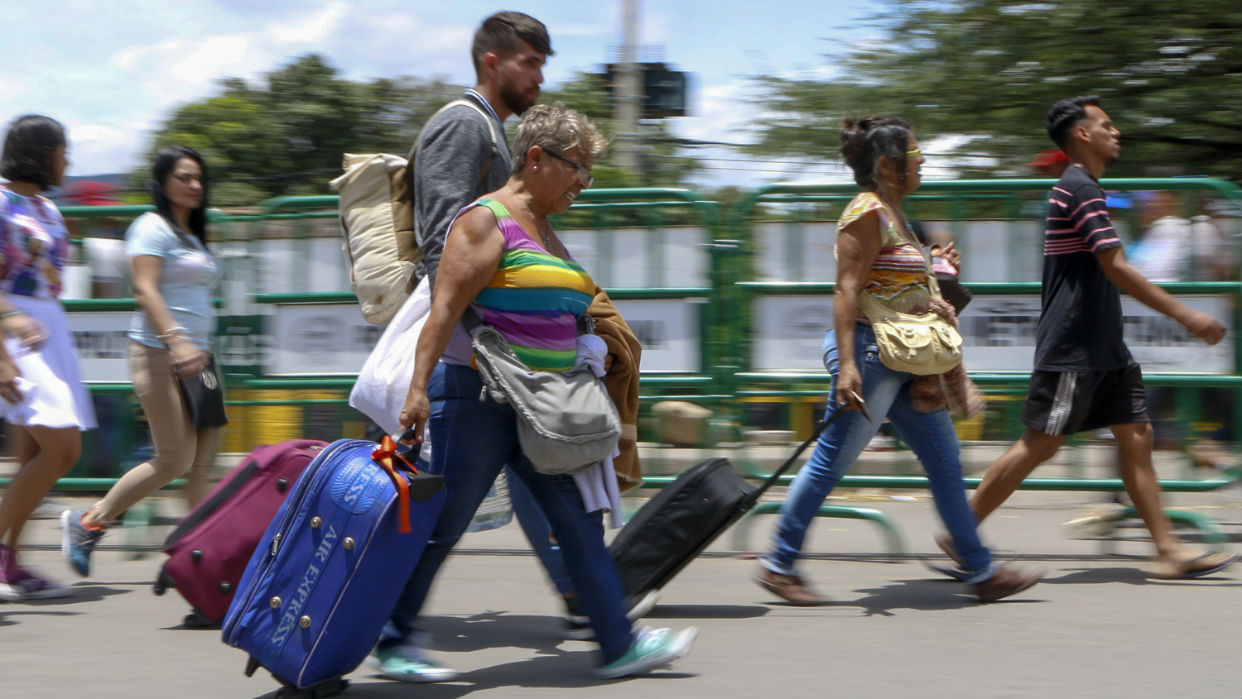
\includegraphics[width=300px]{251.jpg}%
\newline%
%
Ginebra.{-} El Programa Mundial de Alimentos (PMA), el principal brazo humanitario de Naciones Unidas, informó este martes que necesita 22 millones de dólares suplementarios para atender al creciente número de venezolanos que entra a Colombia.%
\newline%
%
"Cuando las familias inmigrantes llegan a los centros de recepción reciben alimentos calientes y pueden quedarse de tres a cinco días, pero luego tienen que irse para que otros recién llegados puedan ser atendidos", dijo el portavoz del PMA, Herve Verhoosel.%
\newline%
%
Muchos de los que tienen que abandonar esas instalaciones temporales se convierten en personas sin domicilio o viven en asentamientos informales que se van creando.%
\newline%
%
Miles de familias venezolanas "viajan días y semanas por rutas peligrosas que pasan ríos, encuentran frecuentemente gente mal intencionada y, en general, no están preparadas para este tipo de travesía", explicó.%
\newline%
%
La falta de alimentos se convierte en el principal problema para quienes atraviesan a diario la frontera entre Venezuela y Colombia, que cuenta con siete puntos de pasaje oficiales y más de un centenar informales, con más del 50\% de inmigrantes que entran a Colombia por estos últimos.%
\newline%
%
El PMA ha proporcionado ayuda alimentaria de emergencia a más de 60.000 venezolanos en los departamentos fronterizos de Arauca, La Guajira y el Norte de Santander, en Colombia, y más recientemente ha empezado también a operar en el departamento de Nariño, que tiene frontera con Ecuador.%
\newline%
%
A petición de la autoridades colombianas, el organismo también desarrollará actividades en favor de la integración de los inmigrantes y la estabilidad de las comunidades que los reciben.%
\newline%
%
"Ante el aumento previsto de inmigración a Colombia, el PMA espera que la comunidad internacional siga apoyando esta respuesta de emergencia", comentó Verhoosel, reseñó Efe.%
\newline%
%
Según recientes evaluaciones efectuadas por el PMA entre inmigrantes en Colombia, el 80\% de ellos sufren de inseguridad alimentaria.%
\newline%
%
\end{document}